\documentclass[prd,floatfix,preprintnumbers,amsmath,amssymb,nofootinbib,superscriptaddress]{revtex4}
\usepackage{graphicx}% Include figure filesg
\usepackage{subfigure}

\def\pheq{\phantom{=}}
\newcommand{\Deqn}[1]{{Eq.~(\ref{#1})}}
\newcommand{\Deqns}[1]{{Eqs.~(\ref{#1})}}
\newcommand{\Ceqn}[1]{{Equation~(\ref{#1})}}
\newcommand{\Dfig}[1]{{Fig.~\ref{#1}}}
\newcommand{\beq}{\begin{equation}}
\newcommand{\eeq}{\end{equation}}
\newcommand{\bea}{\begin{eqnarray}}
\newcommand{\eea}{\end{eqnarray}}
\newcommand{\tr}{{\mathop{\mathrm{tr}}\nolimits}}

\begin{document}


\title{Practicum 4: Digital filtering and correlations}

\maketitle

\section*{Part A: Digital filtering}

We'll start by playing with some digital filters to get intuition 
for how they work. Then we'll design our own. Start up the digital filtering 
java applet (go to http://www.falstad.com/dfilter/, or open it
from the files included in this exercise, i.e. open dfilter/derections.html).

\begin{itemize}

\item In the Java applet, select speech as your input and a low pass FIR filter. 
Set the cutoff frequency to the maximum.  Gradually lower the cutoff frequency.  
Which letters (consonants or vowels) do have more trouble distinguishing as you lower the cutoff?
[This actually poses a challenge for telephone communications... When I travel I sometimes find 
myself with a hotel reservation under Fiemenf instead of Siemens]

\item Keep the the low-pass FIR and set the input to be the triangle wave. Starting from the lowest frequency, 
slowly increase the cutoff frequency letting in one harmonic (spike in the spectrum plot) at a time. 
What's happening to the waveform?  Explain it in terms of what you see in
the spectrum and the Fourier series expansion for a triangle wave (google this if you don't know what it is).

\item Try various filters and inputs with the Java Applet to get more intuition for 
what filtering does to data (white noise is fun).  What happens to the 
frequency response of FIR filters as you increase their order? What 
happens to the frequency response of IIR filters (like the Butterworth filters) 
as you increase the number of poles?

\item Now let's write our own code to generate a digital filter. We'll do this by 
choosing a desired frequency response in the frequncy domain and inverse Fourier transforming to generate a 
filter in the time domain.

\begin{figure}[h]
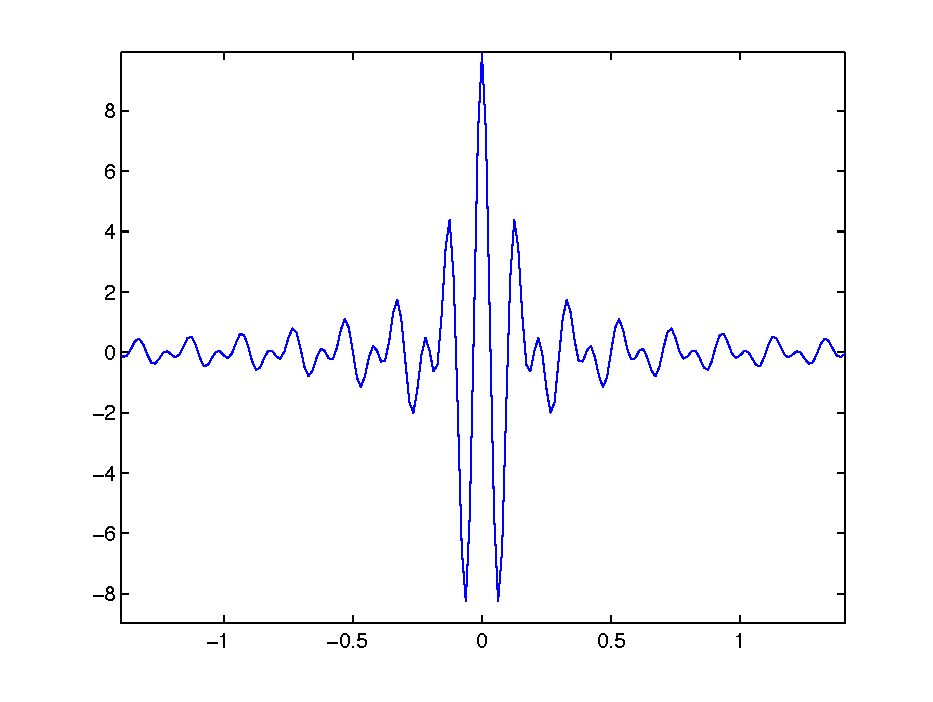
\includegraphics[width=7cm]{filter-square}\\
\caption{Close-up of square time domain filter with sharp edges.}
\end{figure}

\begin{figure}[h]
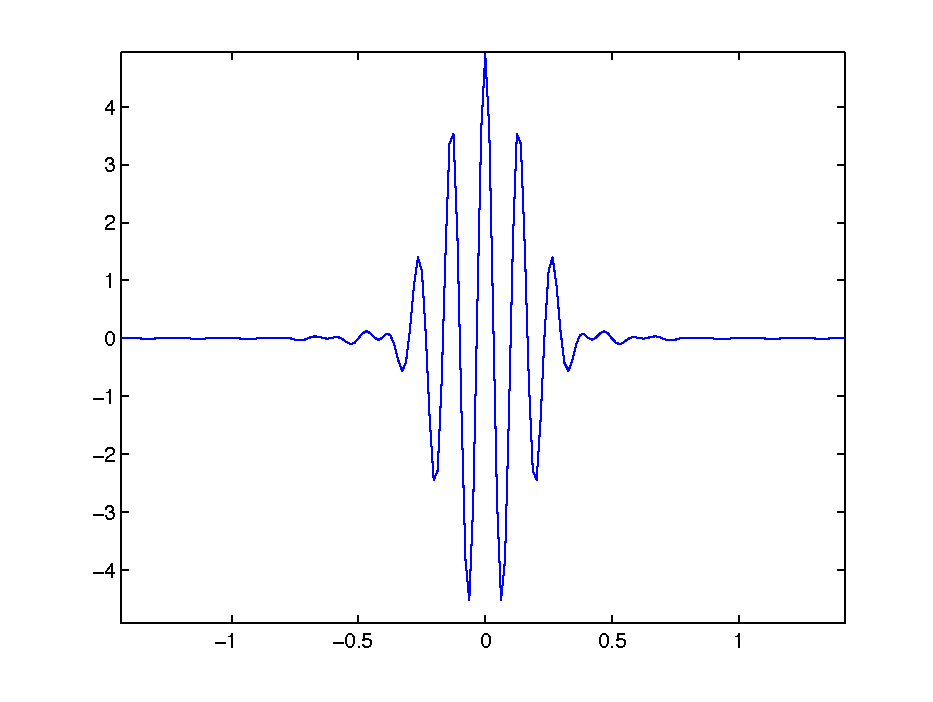
\includegraphics[width=7cm]{filter-hann}\\
\caption{Close-up of square time domain filter with Hann-windowed smoothed edges.}
\end{figure}


\begin{itemize}

\item You have a code that generates a band pass filter with a band-pass between 5Hz-10Hz. Run it 
to produce two plots: a plot of the filter in the frequency domain, and a plot of the filter in the time domain 
(computed via an inverse FFT). The script is pretty well commented, but let us know if you have any questions.

\item If you zoom in on or near the center of the filter (around t=0), you'll notice the filter has a lot of 
time-domain substructure (wiggles). This substructure is a manifestation of the Gibbs phenomenon 
(look it up on wikipedia!). We can get rid of this by removing the discontinuities in the frequency domain response 
at 5Hz and 10Hz, i.e. ramping up the frequency domain response smoothly and then ramping it back down smoothly 
with a window function.

\item Instead of a rectangular window (the sharp cutoffs at 5Hz and 10Hz) use a Hann window defined by 
$$
h(k)=\frac{1}{2} \left[ 1-\cos \left( \frac{2 \pi k}{N-1}\right) \right], 
$$
where $k=0,...,N-1$, is the value of the window at a given data point, and $N$ is the total number of data points. 
Plot the frequency response and the time-domain filter (most of this will be copying and pasting from the code 
you already have).

\item Zoom in to the central part of the filter and notice how all the high frequency structure has disappeared.



\item  You should jump to the next section at this point. If you 
have time later filter some white noise data in the time domain
with your filter and compare spectra of filtered and un-filtered data, to check that 
the right frequency content has been removed.

\end{itemize}

\end{itemize}




\section*{Part B: Correlations}

As part of your materials you have three data sets (each consisting of two sets of data that you will be 
correlating). The correlation $r_{xy}$ between two data series $x$ and $y$ is defined as
$$
r_{xy}=\frac{1}{N}\frac{\sum_{i=1}^N (x_i-\bar x)(y_i-\bar y)}{\sigma_x \sigma_y},
$$
where $\bar x$ and $\sigma_x$ are the mean and standard devitions of the $x$ data 
(similarly for $y$), and $i$ is the index labeling the $N$ points in each time series.

You have three data sets each with two data files: data/dataset1-1.txt and data/dataset1-2.txt; data/dataset2-1.txt 
and data/dataset2-2.txt; and data/dataset3-1.txt and data/dataset3-2.txt. Each of the 
data sets contains 10 years of data, with 500 points total.

\begin{itemize}

\item You have some code that loads the data files for the first 
data set (data/dataset1-1.txt and data/dataset1-2.txt). Add some code that 
computes the correlation as defined by the equation above.

\item Copy and paste this code to do the same with data/dataset2-1.txt and data/dataset2-2.txt 
and data/dataset3-1.txt and data/dataset3-2.txt

\item Compare the values of the cross correlation you obtain for each of the three cases, 
and determine which data sets contain data that is correlated. To do this look at Fig.~3 which 
shows the probability distribution for values of the cross-correlation in the absence of 
correlated noise (assuming the data in both sets is Gaussian and we have 500 points).

\item Plot the three data sets and see if you spot how the pairs are correlated.

\item One possibility is that correlations appear due to the presence of spectral lines, i.e. 
sinusoids in each of the data that are correlated.  First you should check whether there are sinusoids, 
then you can see if the sinusoids are correlated (in phase). How can you check this? 

\item If you have time: Another possibility is that a subset of the data is correlated while 
the rest is not. To check this you can construct a sliding correlation: go though the data 
correlating only the nearest $N_c$ points

\end{itemize}


\begin{figure}[h]
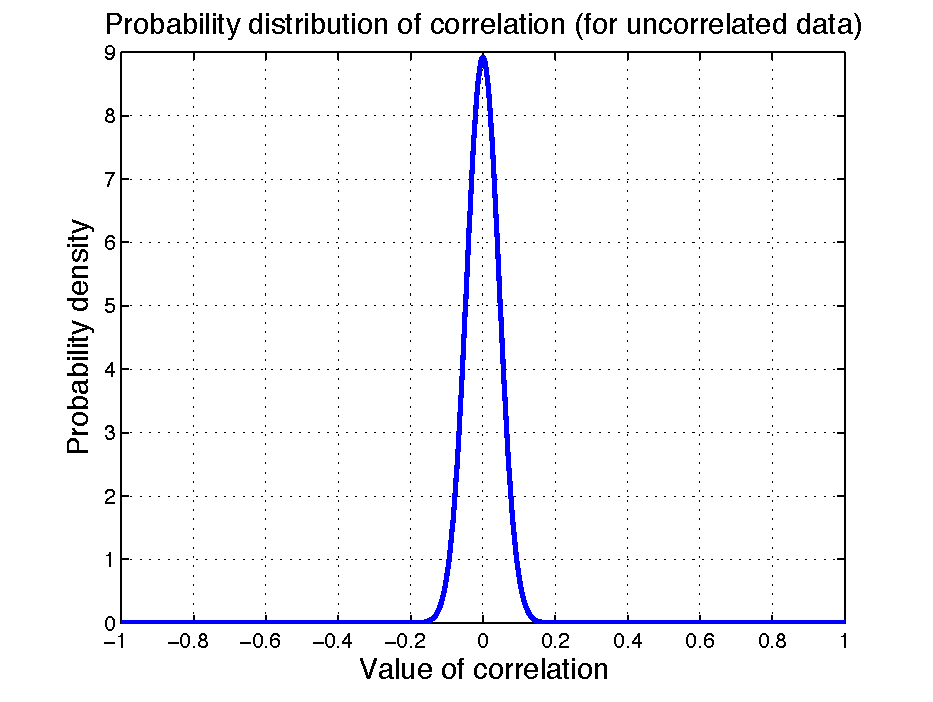
\includegraphics[width=17cm]{pdf}\\
\caption{Probability distribution for the value of the correlation for two data sets each 
consisting of 500 data points of white Gaussian noise.}
\end{figure}

\end{document}
